\documentclass[10pt]{article}
\usepackage[polish]{babel}
\usepackage[utf8]{inputenc}
\usepackage[T1]{fontenc}
\usepackage{amsmath}
\usepackage{amsfonts}
\usepackage{amssymb}
\usepackage[version=4]{mhchem}
\usepackage{stmaryrd}
\usepackage{graphicx}
\usepackage[export]{adjustbox}
\graphicspath{ {./images/} }

\title{II Konkurs matematyczny St@ś }

\author{}
\date{}


\begin{document}
\maketitle
\section*{XIV LO im. Stanisława Staszica \\
 29 maja 2002 roku}
\section*{klasa VI}
Na rozwiąanie poniższych zadań masz 90 minut. Kolejność rozwiqzywania tych zadań jest dowolna.\\
Wszystkie zadania sq jednakowo punktowane. Maksymalnq liczbę punktów może uzyskać jedynie pelne rozwiqzanie, z uzasadnieniem i odpowiedzia.\\
Uzywanie korektora i korzystanie z kalkulatora jest niedozwolone.

\section*{Zadanie 1.}
Klasa licząca 27 uczniów kupiła na loterii losy z numerami od 1 do 27 . Każdy uczeń wylosował jeden los, a następnie dodał numer swojego losu do swojego numeru w dzienniku. Uzasadnij, że \({ }^{-\bullet}\) przynajmniej jeden uczeń otrzymal w wyniku tego dodawania liczbę parzysta.

\section*{Zadanie 2.}
Podaj wszystkie takie liczby \(x\), dla których iloraz \(\frac{15}{x-4}\) jest liczbą całkowitą ujemną.

\section*{Zadanie 3.}
Odpowiedz na poniższe pytania:\\
a) Czy \(17 \%\) dwucyfrowej liczby naturalnej może być liczbą naturalną? Dlaczego?\\
b) Czy 22\% dwucyfrowej liczby naturalnej może być liczbą naturalną? Dlaczego?

\section*{Zadanie 4.}
Naszkicuj i opisz przykład czworokąta, który jednocześnie spełnia następująe dwa warunki:

\begin{enumerate}
  \item czworokąt ten nie jest rombem,
  \item każda przekątna dzieli ten czworokąt na dwa trójkąty równoramienne.
\end{enumerate}

\section*{Zadanie 5.}
Dwa wierzchołki graniastosłupa prostego pięciokatnego oznaczono literami \(A\) i \(B\). Następnie rozcięto ten graniastosłup i otrzymano jego siatkę.\\
Na narysowanej siatce oznacz literą \(A\) wszystkie punkty, które były sklejone z wierzchołkiem \(A\), a literą \(B\) oznacz wszystkie punkty, które były sklejone z wierzchołkiem \(B\).\\
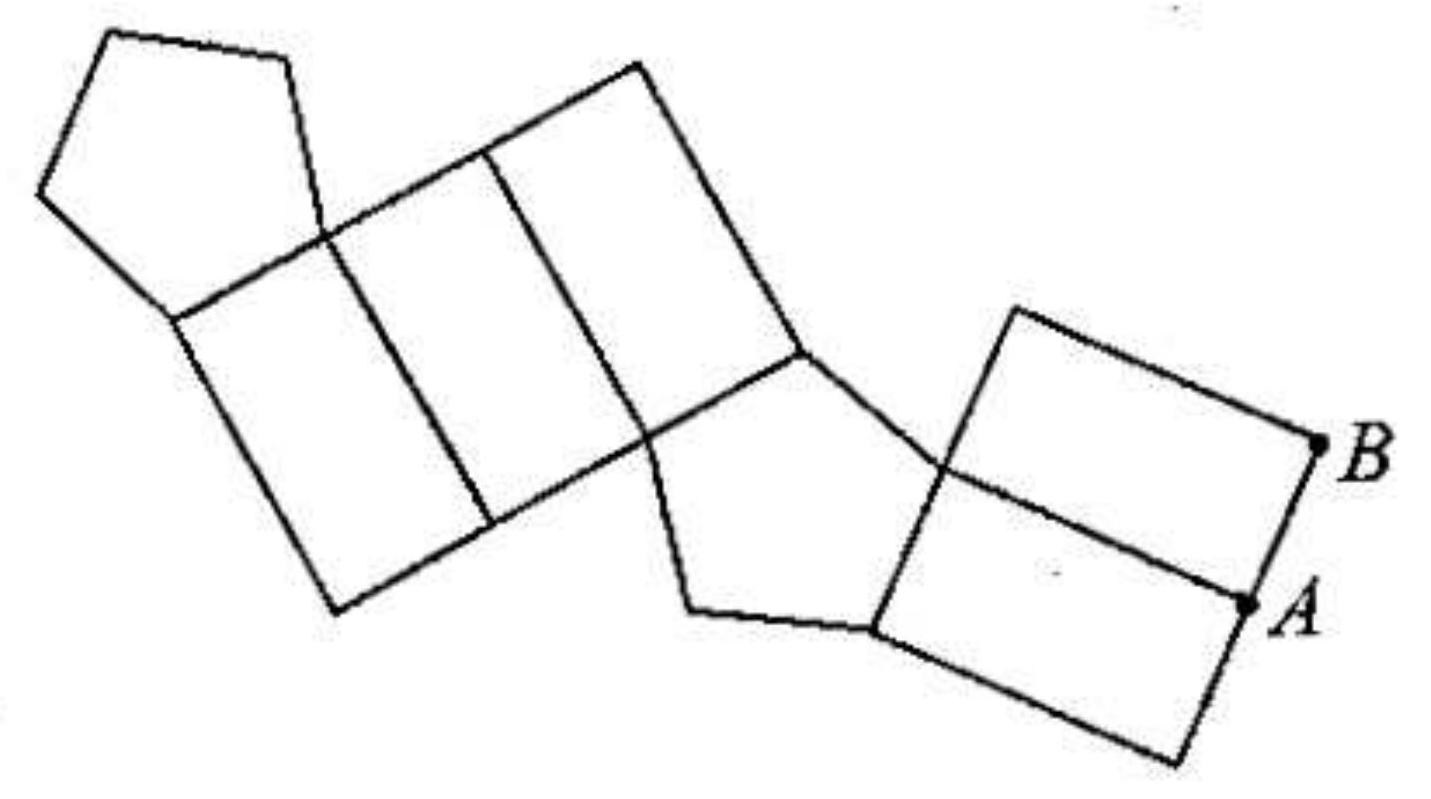
\includegraphics[max width=\textwidth, center]{2024_11_21_3a60c5cfbd5f3f387295g-1}


\end{document}